%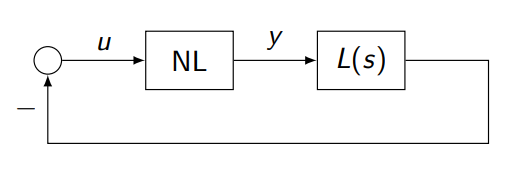
\includegraphics[width = \linewidth]{src/images/nolinearity_block_diagram.png}
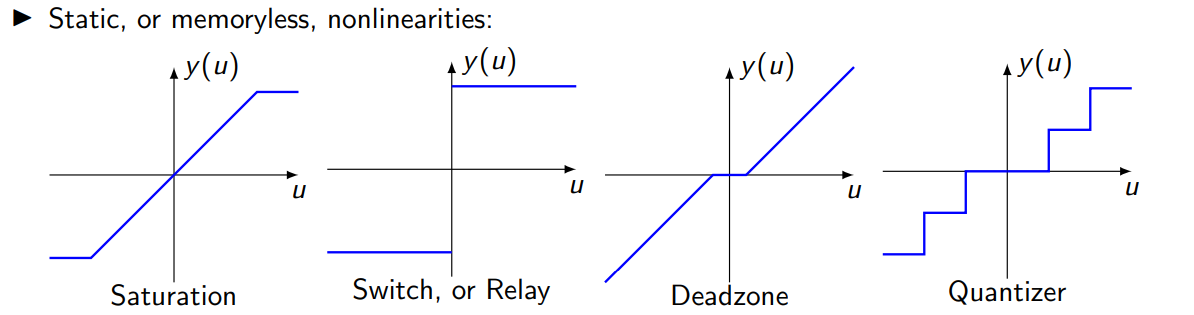
\includegraphics[width = \linewidth]{src/images/nonlinearity_example.png}
\begin{minipage}{0.29\linewidth}
    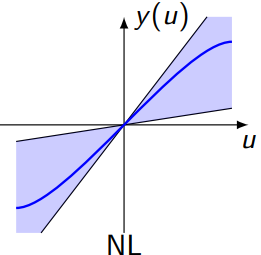
\includegraphics[width = \linewidth]{src/images/nolinearity_plot.png}
\end{minipage}
\begin{minipage}{0.29\linewidth}
    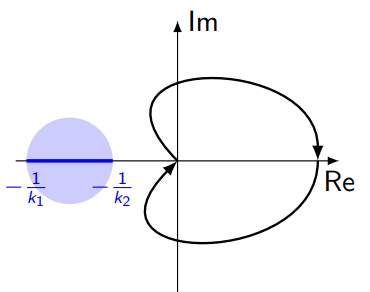
\includegraphics[width = \linewidth]{src/images/nolinearity_nyquist.png}
\end{minipage}
\begin{minipage}{0.39\linewidth}
    Nonlinearity bounded by linear functions with slope $k_1$ and $k_2$
\end{minipage}

Nyquist condition now applies to a circle.\\
Necessary condition: For some of the given nonlinearities, the system is stable (Nyquist plot can go through the circle)\\
Sufficient condition: For all of the given nonlinearities, the system is stable (Nyquist plot does not go through the circle)

\subsection{Describing Function}
    %Every Output $y(t)$ with a sinusodial input function $u(t) = A \sin(\omega t)$ can be written as a fourier series:
    %\begin{align*}
    %    y(t) = \frac{a_0}{2} + \sum\limits_{i = 1}^{\infty}[a_i \cos(i \omega t) + b_i \sin(i \omega t)]\\
    %    a_i = \frac{1}{\pi} \int\limits_{-\pi}^{\pi} y(t) \cos(i \omega t) d(\omega t)\\
    %    b_i = \frac{1}{\pi} \int\limits_{-\pi}^{\pi} y(t) \sin(i \omega t) d(\omega t)
    %\end{align*}
    %For odd nonlinearity y: $a_i = 0$\\
    %We are interested in the first harmonic of an odd function. Therefore 
    %\begin{align*}
    %    \text{describing function: } 
    %\end{align*}
    Output $y(t)$ for $u(t) = sin(\omega t)$ can be approcimated by Fourier\\
    if nonlinearity is odd and static: $a_n = 0$ in Fourier\\
    We are only interested in first harmonic: $y(t) \approx b_1 sin(\omega t)$\\
    Therefore, we define the describing function:
    \begin{align*}
        N(A) = \frac{b_1(A)}{A} = \frac{1}{\pi A} \int\limits_{-\pi}^{\pi} y(t) \sin(i \omega t) d(\omega t)\\
        NL \cdot L(s) \approx N(A) L(s)
    \end{align*}

    \titel{approximate describing function}
    \begin{align*}
        u(t) = Ae^{j \omega t} \Rightarrow
        y(t) \approx c_1(A, \omega) e^{j(\omega t + \phi_1(A, \omega))}\\
        N(A, \omega) = \frac{c_1(A, \omega)}{A} e^{j \phi_1(A, \omega)}
    \end{align*}

\subsection{Stability analysis of nonlinear systems}
    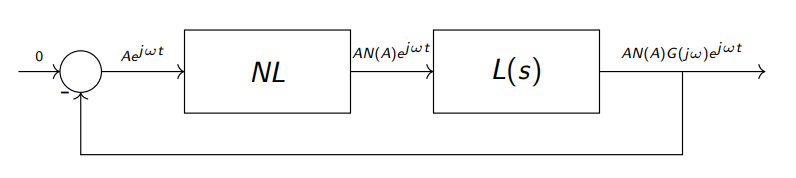
\includegraphics[width = \linewidth]{src/images/nonlinear_stability_block_diagram.png}
    Self sustained oscillation $\Leftrightarrow$ $r(t) = y(t)$ $\Leftrightarrow$ limit cycles
    

    \begin{minipage}{0.54\linewidth}
        \begin{align*}
            A e^{j \omega t} &= A \cdot N(A) \cdot L(j \omega) e^{j \omega t}\\
            &\Leftrightarrow - \frac{1}{N(A)} = G(j \omega)
        \end{align*}

        
        In Nyquist:\\
        Possible limit cycles at Nyquist intersection of $- \frac{1}{N(A)}$ and $G(j \omega)$\\
        
        
        $-\frac{1}{N(A)}$ point in “unstable” region: $A$ increases\\
        
        
        $-\frac{1}{N(A)}$ point in “stable” region: $A$ decreases
    \end{minipage}
    \begin{minipage}{0.44\linewidth}
        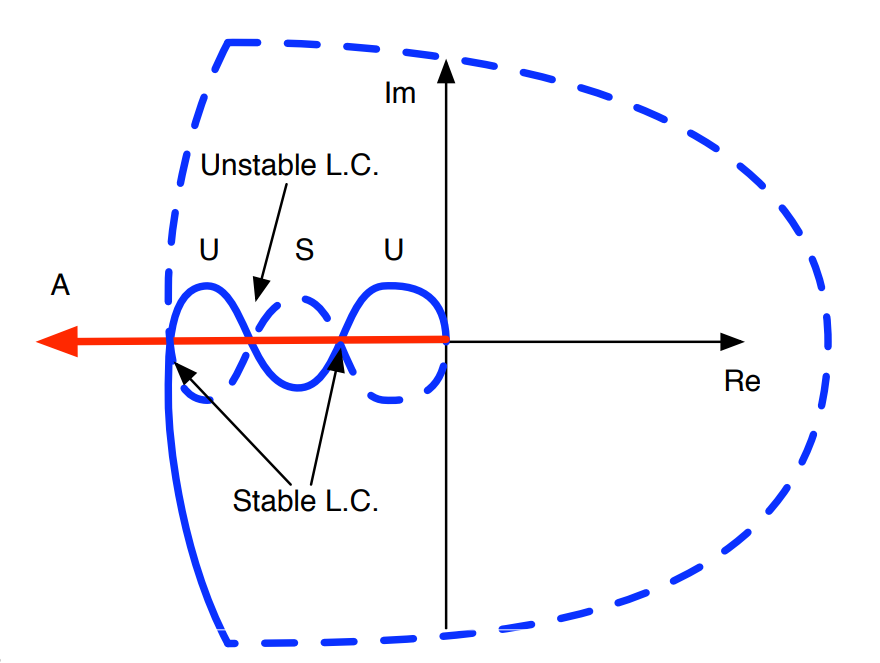
\includegraphics[width = \linewidth]{src/images/nonlinearity_stability_limit_cycles.png}
    \end{minipage}
    
